\section{Termine}

\begin{figure}[b]
  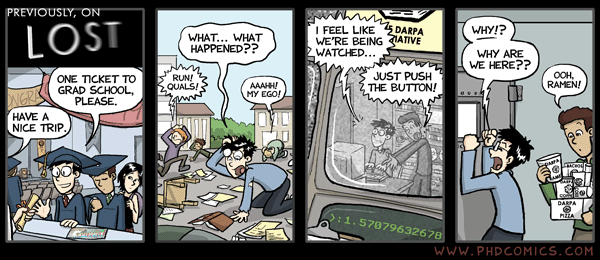
\includegraphics[width=\textwidth ]{bilder/comics/phd092706s.png}
\end{figure}

Gerade in der Anfangszeit des Studiums gibt es eine Menge zu tun. Damit ihr
nicht das Wichtigste verpasst, haben wir die ersten Termine kompakt f"ur
euch zusammengefasst. Die meisten davon bieten die Gelegenheit Fragen zu
stellen und nebenbei gleich ein paar nette Kommilitonen kennen zu lernen.

Das K"urzel nach Datum und Zeit gibt den Raum bzw. Ort an. F"ur alle R"aume die nicht
im IZ (steht f"ur Informatikzentrum) liegen, schaut am besten auf den
Raumplan. Bei den R"aumen im IZ ist die erste Zahl das Stockwerk, f"ur
den Rest m"usst ihr dann auf den Plan im Stockwerk schauen (Kleine Falle:
zwischen EG und 1. OG liegt das Galeriegescho"s - Raum 149/150 liegt also
effektiv in der zweiten Etage).\par

\begin{description}
  \item[Mo, 29.09. -- Do, 2.10. ~~ 13 Uhr] \hfill \nroom{SN 19.1} \\
  Vorkurs Informatik
  \nurlfootnote{http://www.ips.cs.tu-bs.de/content/view/192/30/lang,german/}
  \item[Mo, 6.10. -- Fr, 17.10. ~~ 9 Uhr] \hfill \nroom{Audimax} \\
  Vorkurs Mathematik
  \item[Mo, 20.10. -- Fr, 24.10.] \ \\
  Vorkurs Informatik\footnotemark[1]
  \item[Mi, 22.10. ~~ 16 Uhr] \ \\
  Infoveranstaltung der FG \\
  \item[Mo, 27.10. ~~ 9 Uhr] \hfill \nroom{Audimax} \\
  Begr"u"sung durch Pr"asidenten \& AStA
  \item[Mo, 27.10. ~~ 10 -- 12 Uhr] \hfill \nroom{Foyer Altbau} \\
  Infob"orse ,,Studium ist mehr ...''
  \item[Mo, 27.10. ~~ 14 -- 15 Uhr] \ \\
  Begr"u"sung durch die Dozenten
  \item[Mo, 27.10. ~~ 15 Uhr] SN 19.1 \\
  1. Vorlesung ,,Programmieren I''
  \item[Mo, 27.10. ~~ 16.30 Uhr] SN 19.1 \\
  Grillen der FG Informatik
  \item[Mo, 27.10. ~~ ab 21 Uhr] \hfill \nroom{Audimax} \\
  Erstsemesterparty
  \item[Di, 28.10. ~~ 10 Uhr] \hfill \nroom{Plaza im IZ} \\
  Erstsemesterfr"uhst"uck
  \item[Di, 28.10. ~~ 11 Uhr] \hfill \nroom{Plaza im IZ} \\
  Infoveranstaltung der FG \\
  Einteilung in die Tutorengruppen \& F"uhrung "uber den Campus
  \item[Mi, 29.10. ~~ ab 10 Uhr] \ \\
  ,,Studium Generale''
  \item[Mi, 12.11. ~~ ab 19 Uhr] \hfill \nroom{IZ 150} \\
  Spieleabend der Fachgruppe
\end{description}


% - Erig-Party im AM
% - Gl"uhweinabend im Informatikzentrum (IZ)